\chapter{Architecture}

While the fundamental goal of libbind \todo[inline]{we likely will rename this later} is to provide static detouring, the usefulness of such a feature is greatly diminished without appropriate supporting functionality. If a user was required to provide raw addresses to patch, the library would not be usable standalone. This section discusses the architecture of the library and presents its constituent components. The actual implementation will be covered separately so there may be minor inaccuracies and inconsistencies for the purpose of simplicity. 

The following diagram illustrates the three main components of libbind:

\begin{figure}[H]
 \centering
 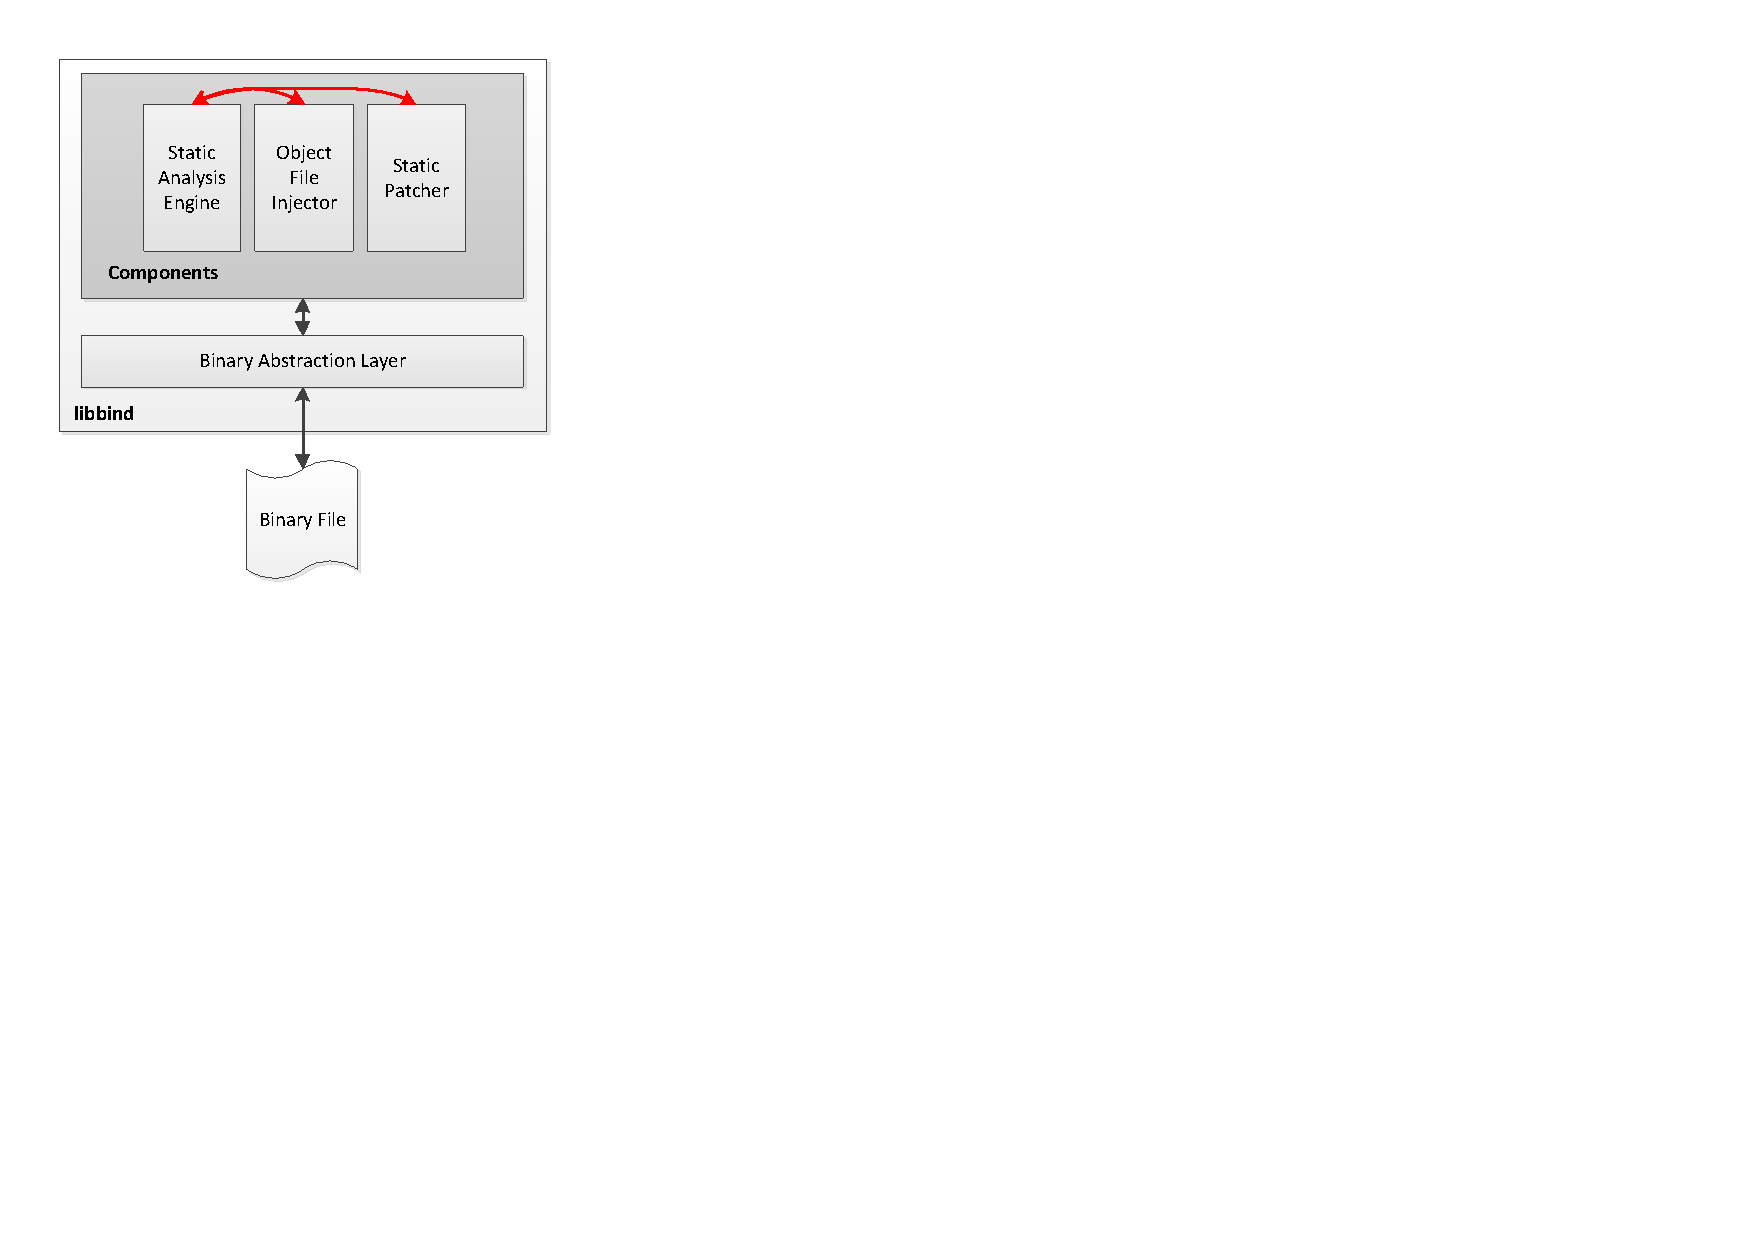
\includegraphics{Architecture.pdf}
 \caption[Architecture]{The high level architecture of libbind}
\end{figure}

As defined in \emph{(F4)} and \emph{(F5)} of the specification, we have chosen to treat the code of a binary as a CFG. As such, any modifications to the code of a binary are done so through the addition, deletion or modification of nodes/vertices in the CFG. Hence, a simplified and abstract way of considering each component of libbind is in terms of the operations it performs upon the CFG.

\section{Static Analysis Engine}

\begin{figure}[H]
 \centering
 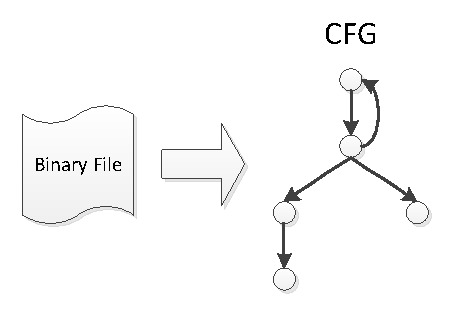
\includegraphics{Static_Analysis_Engine.pdf}
 \caption[Static Analysis Engine]{The primary role of the static analysis engine is to generate the CFG.}
\end{figure}

The primary role of the disasm engine is to generate the inital CFG. 

 we view the code of the binary as a CFG, the role of the disasm engine is to generate that CFG. the role of the object file injection is to extend that CFG such that the cfg after injection is a superset of the cfg before injection (add a set of nodes and edges disjoint to the original cfg). the role of the static patcher is to 

 The fundamental goal of the library is to provide static detouring, the other components of the library largely play a supporting role. one key aspect of the library that should be noted is the support for both x86-32 and x86-64. the high level of architectural similarity means there is a large degree of overlap in code dealing with these architectures. however, the library often branches off to architecture specific 

during our discussion of the library architecture, we will abstract away from these issues. the specifics will be covered in details in 'implementation'.

architecture
- disasm engine
  - symbol table representation
- object file injection
- static patcher

the reasons for this separation are:
- a natural and inherent separation in duty between these three parts
- while we can provide interoperability between these components through a well-defined interface but the decoupling allows the implementation to be changed and different implementations 'plugged in'

disasm engine
- even though static patcher is focus of the library, by itself, it is not useful. static patcher provides useful functionality, but if the user is required to provide raw addresses to patch, our library would not be usable standalone
- need to generate an internal representation of a binary. generate an internal CFG (define CFG here). so we have a list of connected functions (composed of basic blocks). exposing an interface to the CFG lets a user locate and express the source and destination for static patching.
- one way they can do this is by specifying a heuristic in terms of instructions and iterate all basic blocks till they find a match. for example:

-- let's also define what a basic block is here

  for\_each\_bb(...) {
    if(bb[0] == push andand bb[0].operand1 == ebp andand bb[1].operand2 == esp)
    ... {
      detour(bb, ...)
    }
  }

verbose but necessary in order to be able to search at instruction granularity. a more useful way to locate functions/basic blocks is through the symbol table which is a valuable resource if available.
- disasm engine parses symbol table and stores this information alongside the cfg. the above example, with symbol information any interactions with the function could be expressed alternatively in a far easier way:
  bf\_basic\_blk * bb = find\_symbol\_by\_name(...);
  detour(bb, ...)

the functionality the disasm engine provides is powerful and can conveniently be used in many other applications. most notably it is possible to do static analysis by comparing the cfg of two binaries. this is not functionality that is provided by libbind which is a general purpose library but is one alternative application. we demonstrate this as part of the evaluation.

object file injection

...

static patcher

the role of the static patcher is to take a binary which is assumed to have all necessary code and 

IMPLEMENTATION
disasm engine builds on top of several abstractions. detailed diagram of disasm engine and how it works above libbfd and libopcodes. perhaps some justification for why we chose to use these

in practice, the disassembler engine is responsible for parsing and translating the strings received from libopcodes and storing that information in its internal semantic representation (bf\_insn, bf\_basic\_blk). bf\_func can be identified from three ways only:
1) if it is the target of a call site
2) if it corresponds to an address identified as a bf\_sym
3) if the user defined it as a root for cfg generation and explicitly stated it is a function (cfg analysis and generation is covered in depth in...)

further information such as size of symbols (which tells us size of function) is available because we are parsing the symbol table directly from libelf.

quirks of libopcodes disassembler such as how it passes us the instruction parts (mnemonic, operands, separator) as strings! we build a finite state machine which allows us to 

we can draw finite state machine in diagram here

binary\_file

within a binary\_file, there are 2 levels of code representation. firstly we have bf\_basic\_blk which represents a basic\_block as defined in architecture.

binary\_file is composed of a CFG of bf\_basic\_blk objects. during the process of cfg generation and after it completes, we add extra information. i.e., bf\_func 'labels'

bf\_func

implementation of CFG analysis and generation...

distribution and documentation

automake which we use to deal with library dependencies (libelf, libbfd, libopcodes, libkern).

 and doxygen

WORKFLOW



TESTING

we want to test robustness and reliability of the library. several areas in particular:

- we want make sure the library is scalable and does not fail on large scale systems. we test on real-world systems, as opposed to toy examples. namely, we test against coreutils (includes stuff like ls, cp, rm, etc.).

we have a suite of regression tests which test the following:

test 1: coreutils\_test32/64

so firstly we want to test the successful disassembly and cfg generation for some real-world example. 

probably want to use valgrind to check for errors